% \subsection{Neural Network}


The accuracies of our models %the model for DIA and no\diabased\  using the $80,000$ for training and the $20,000$ for testing 
are presented in \autoref{tab:acc results}. The \diabased\ model reached, by design, the accuracy of our benchmark model \texttt{autoscan}: ~97\% on True Negative (TN) rate and 95\% on True Positive (TP) rate (see \autoref{sec:method}). We remind the reader that we use the \texttt{autoscan} convention for the definition of TN and TP: Positive is a ``real'' transient ($\texttt{label = 0}$), negative is a ``bogus'' ($\texttt{label = 1}$). There is a drop of $\sim 4\%$ between the accuracy of the \diabased\ and the \nodia\ models. Along with the accuracy, in \autoref{tab:acc results} we present computational costs of training on 20,000 images measured in CPU Node hours,\footnote{The computational cost was calculated by using the formula given in \url{https://docs.nersc.gov/jobs/policy/} and the allocations information given by the system Iris \url{https://iris.nersc.gov}. Training time is reported in CPU hours. Prediction time is reported per “postage stamp” (1ms) and the classification operation is trivially parallelizable (can be run independently on each postage stamp).} and the clock time for the prediction for one single image.


\begin{table}
\footnotesize{
    \centering
    \begin{tabular}{|c|c|c|c|c|}
    \hline
    \multirow{2}{*}{\bf{Model}}& \multicolumn{2}{c|}{\centering \bf{Accuracy}}
 & \bf{Train time}$^7$ & \bf{Prediction}$^7$\\
    \bf{ }&\bf{Train} & \bf{  Test} & \bf{(CPU hours)} & \bf{(Clock-time, ms)}\\
    \hline
       \multirow{2}{*}{ \diabased}&\multirow{2}{*}{0.962}&$0.959\pm$&\multirow{2}{*}{$\sim$35}&\multirow{2}{*}{$1.00\pm0.03$}\\&&$0.004$&&\\ \hline
      \multirow{2}{*}{ \nodia}&\multirow{2}{*}{0.915}&$0.916\pm$&\multirow{2}{*}{$\sim$56}&\multirow{2}{*}{$0.30\pm0.01$}\\&&$0.007$&&\\ \hline
    \end{tabular}
    \caption{Comparative table of the accuracy and computational cost for both training and testing data for the \diabased\  (\autoref{fig:architecturesCNN}, left) and \nodia\  (\autoref{fig:architecturesCNN}, right) models. }
    \label{tab:acc results}}
\end{table}
% The accuracy of the model for \diabased\  input data for training and testing data was respectively: \mintinline{c}/Training accuracy: 0.9620/
% \mintinline{c}/Testing accuracy: 0.9590/. The accuracy of the model for no\diabased\  input data for training and testing data was respectively: \mintinline{c}/Training accuracy: 0.9147/
% \mintinline{c}/Testing accuracy: 0.9155/. 
% Using the $80,000$ for training and the $20,000$ for testing. \autoref{fig:loss_modelAAAD} and \autoref{fig:loss_modelCCC} show the loss and the accuracy through the epochs for the \diabased\  model (\autoref{fig:architecture_NN}) and no\diabased\  model (\autoref{fig:architecture_2DNN}) respectively.





% \begin{figure*}
% \begin{minipage}[b]{0.45\linewidth}
%     \centering
%     \includegraphics[width=1\linewidth]{
%     figures/lossacc_modeloverleaf_scale(1).pdf}
%     \caption{\textbf{\diabased\ } loss (top) and accuracy (bottom) for the model described in left \autoref{fig:architecturesCNN}. Purple line represent the validation data (20\% or 20,000 images) and the green the training data (80\% or 80,000 images).}
%     \label{fig:loss_modelAAAD}
% % \end{figure}
% \end{minipage}
% \begin{minipage}[b]{0.45\linewidth}
%     \centering
%     \includegraphics[width=1\linewidth]{
%     figures/lossacc_modeloverleafCCC_scale(1).pdf}
%     \caption{\textbf{\nodia\ } loss (top) and accuracy (bottom) for the model described in right \autoref{fig:architecturesCNN}. Purple line represent the validation data (20\% or 20,000 images) and the green the training data (80\% or 80,000 images).}
%     \label{fig:loss_modelCCC}
%     \end{minipage}
% \end{figure*}


% \begin{minted}{python}
% Training accuracy: 0.9892
% Testing accuracy: 0.9726
% \end{minted}

% The accuracy and loss plot for training and validation data:
% \begin{figure}[hbt!]
%     \centering
% \begin{minipage}{.4\textwidth}
% \centering
%     \includegraphics[width=1\linewidth]{
%     figures/lossacc_modelAAAD_3s\diabased\ H.pdf}
% %    \caption{Accuracy from training and testing data from the initial model.}
%     %\label{fig:accuracyinitialmodel}
% \end{minipage}%
% \begin{minipage}{.4\textwidth}
% \centering
%     \includegraphics[width=1\linewidth]{
%     figures/lossacc_modelCCC_3s2DH.pdf}
%     %\caption{Loss from training and testing data from the initial model.}
%     \label{fig:lossinitialmodel}
%     \end{minipage}%
%     \label{fig:acclossinitialmodel}
%     \caption{Accuracy and loss from the training and validation data for a set of composed by $1106$ transients, $555$ labeled as ``real'' and $551$ as ``bogus''. The data is evaluated in the Neural Network model.}
% \end{figure}



Confusion matrices for the testing set are shown for the \diabased\ model in left panel of  \autoref{fig:confusiomatrix_models} and for the \nodia\ model in the right panel of the same figure. In this figure, as in the following confusion matrices and histograms that we will present in \autoref{subsec: saliency}, correct predictions are indicated in shades of blue, incorrect in shades of orange, and darker shades are associated with the true labels. The percent accuracy for each class, True Positives (TP), True Negatives (TN), False Positives (FP), and False Negatives (FN), as well as the number of images in each class are reported within the figure.  



The Receiver Operating Characteristic (ROC) curve shows the relation between the True Positive Rate (TP / (TP + FN)) also know as recall, and the False Positive Rate (FP / (FP + TN)) when changing the threshold value (\eg, a threshold of 0.5 will indicated that values greater than 0.5 would be classified as ``bogus''). The ROC for the testing data for the \diabased\ and \nodia\ models are presented in \autoref{fig:roc_models}. The Area Under the Curve (AUC), which can be used as a comprehensive metric of the aggregated classification performance of a model \citep{hanley1983method, hernandez2012unified}, is 0.992 and 0.973 for the \diabased\  and \nodia\ models respectively, demonstrating good performance for both models.


The loss and the accuracy curves in the left panel of \autoref{fig:loss_models} for the \diabased\  model shows some evidence of overfitting (the validation curve flattens compared to the training curve) starting just a few epochs before training came to end of the 400-epochs; meanwhile, for the \nodia\ model in right \autoref{fig:loss_models}, after $700$ epochs there was no visual evidence of overfitting indicating that the model is still learning generalized information from the data; yet the accuracy improvements from epoch $400$ to $700$ were small.

The nature of the \nodia\ model leads to hypothesize that because the input data contains less information, this model takes longer to learn features from the data to be able to classify them. The \nodia\ model took in fact longer (more epochs) to come to stable accuracy and loss values. The loss and accuracy curves are also noisier for the validation of the \nodia\ model in right \autoref{fig:loss_models} compared to the \diabased\ model. This also can be explained with the same argument: the \nodia\ model had a harder problem to solve and its learning is less linear. We cannot however rule out, and in fact we suspect, that the hyperparameters or the architecture selected for the \nodia\ CNN model could be improved --- as this is a proof of concept paper and the architecture was chosen to enable a direct comparison with the \diabased\ model, future work will include experimenting with different architectures and an extensive grid-search to optimize hyperparameters.
\begin{figure*}
    \centering
    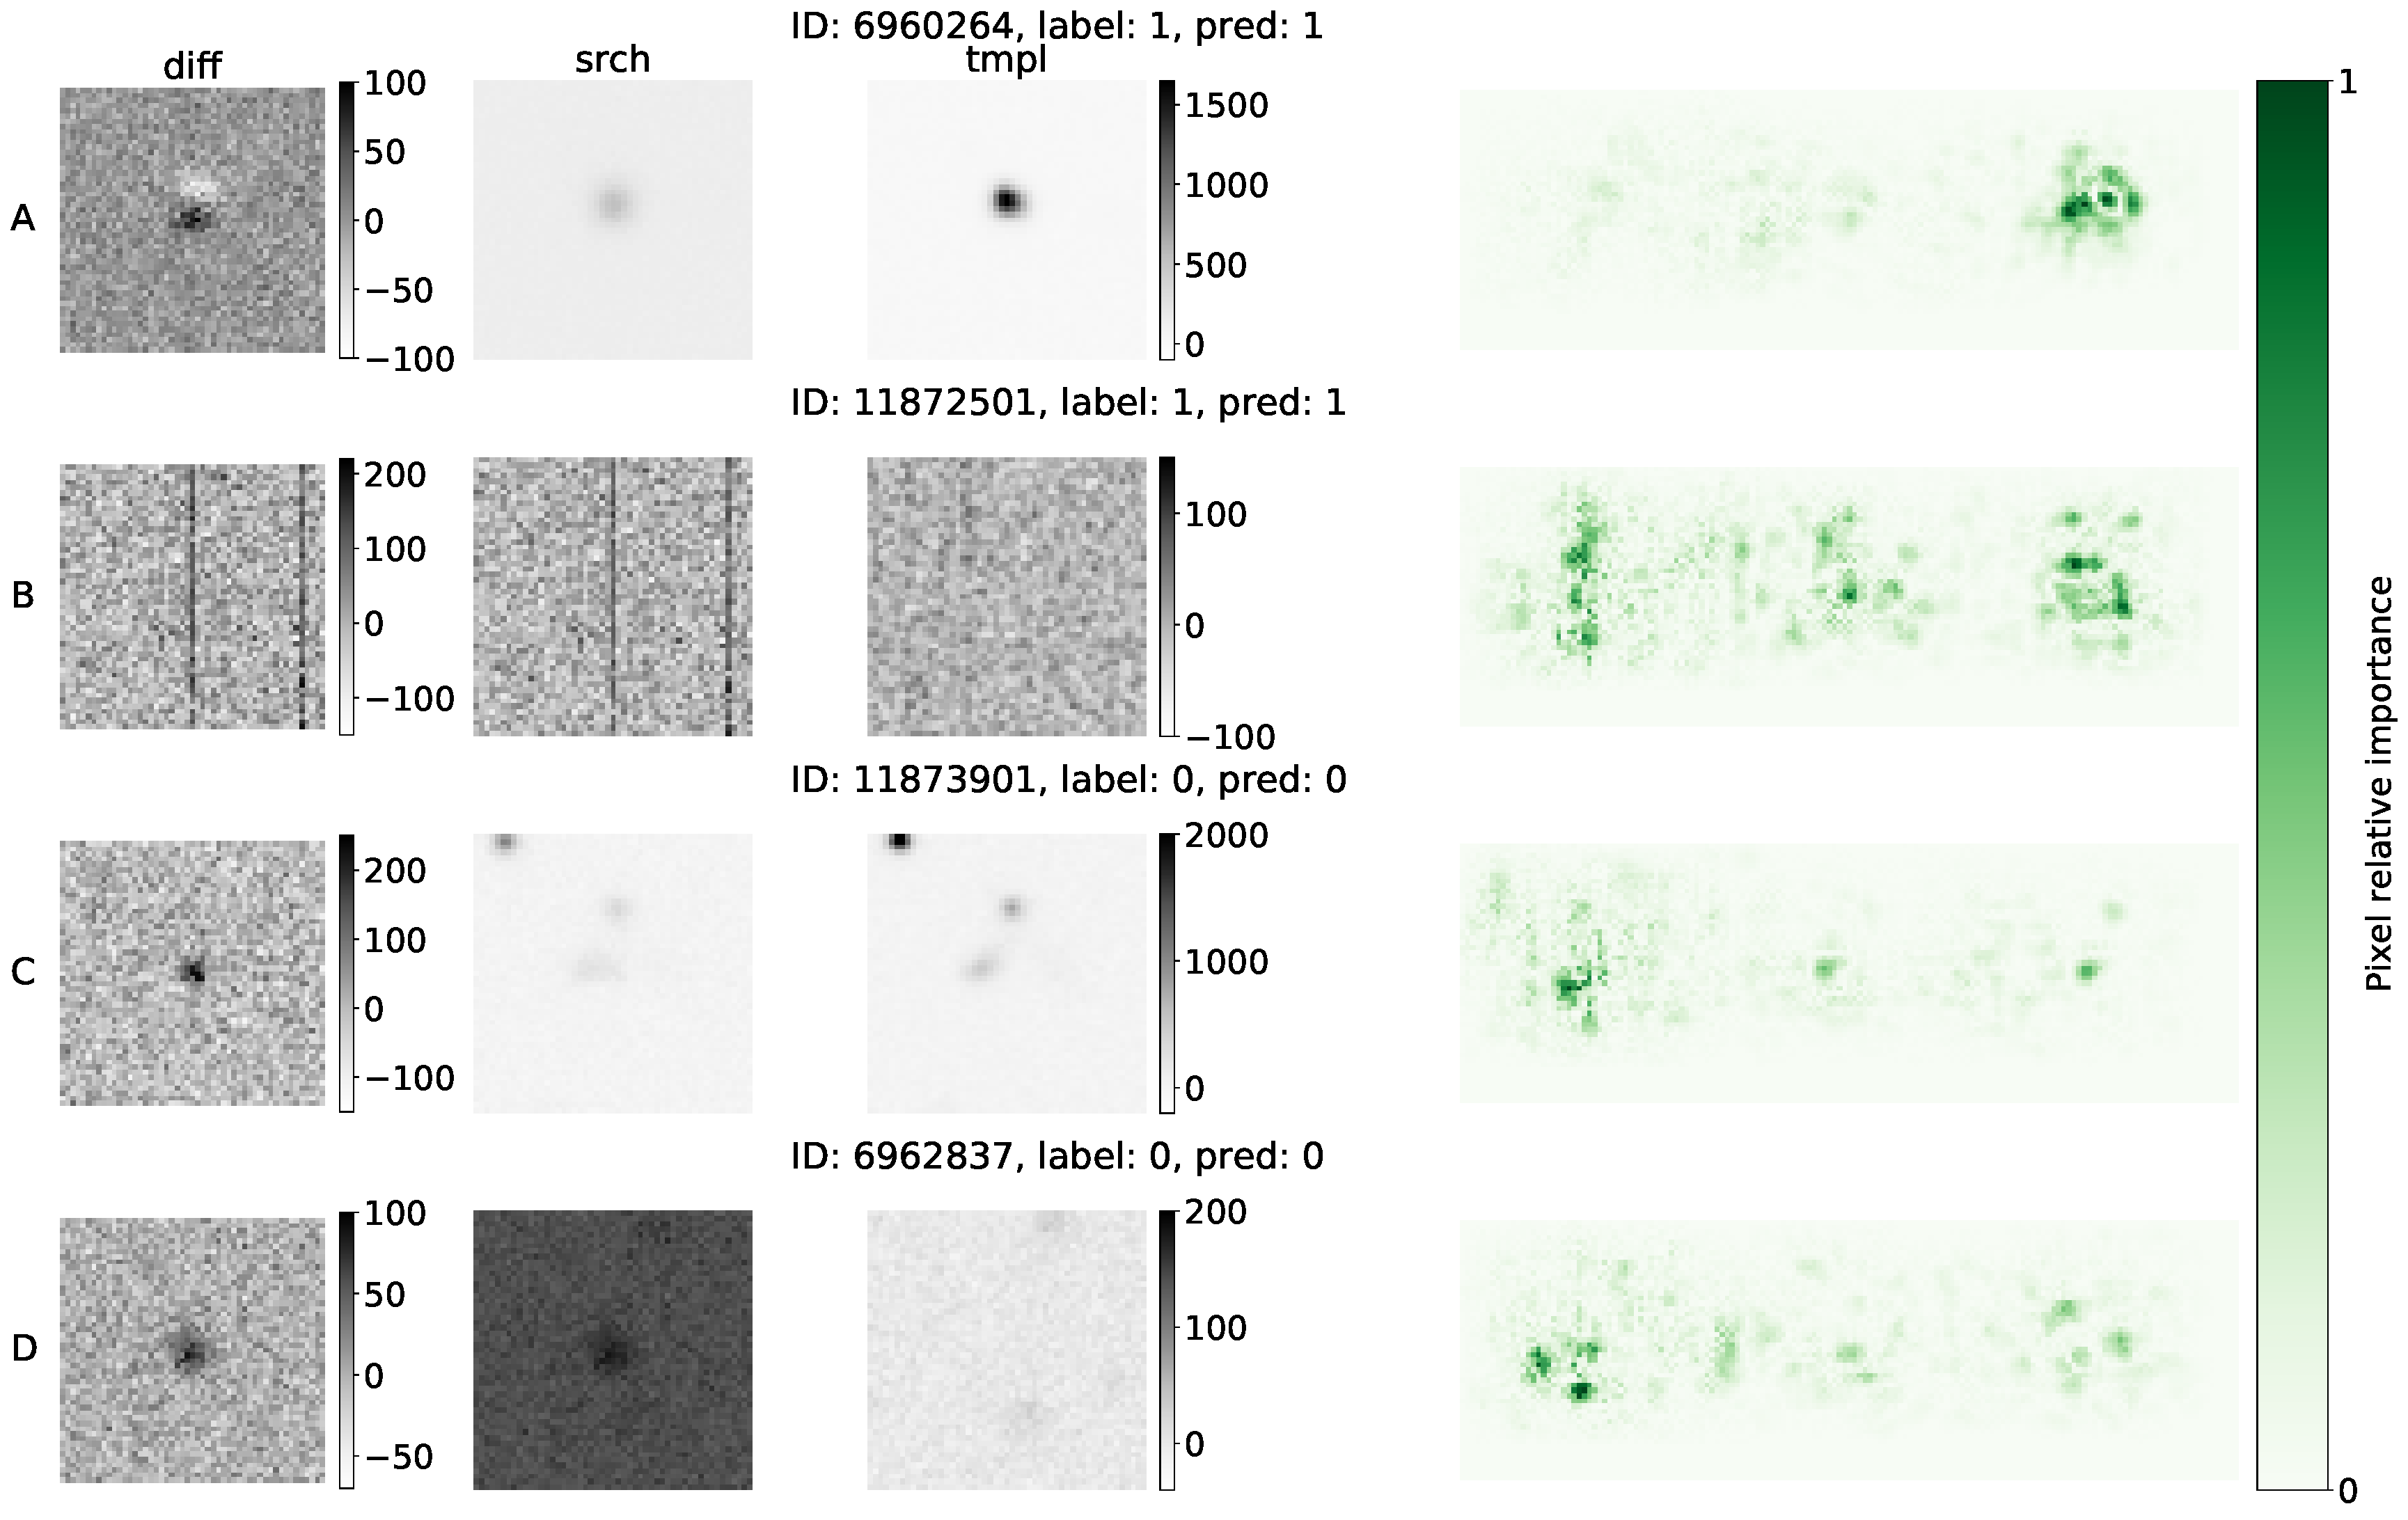
\includegraphics[width=0.9\linewidth]{
    figures/saliency_plot.pdf}
    \caption{Saliency map for the four transients in \autoref{fig:examples_no_normalization} for the \diabased\ model. On the left, in grey color, the original \diff, \search, and \temp\ images are plotted in their natural flux scale (before normalization). On the right, the saliency map for the combined image. The intensity of a pixel color in the white-to-green scale indicates the pixel relative importance: the maps are normalized to 1 individually, such that dark green corresponds to high saliency score, with 1 corresponding to the most important pixel in the image triplet. With the side-by-side organization of the input data, these maps enable a visual understanding of the importance of each element of the combined image in the real-bogus classification. We note how in some cases (panel A) the decision is largely based on the \temp, rather than the \diff\ image, and in some cases all three image elements contribute similarly to the decision (panel B). This figure is discussed in more detail in \autoref{subsec: saliency}.}
    \label{fig:saliency_4id}
\end{figure*}

\begin{figure*}
    \centering
    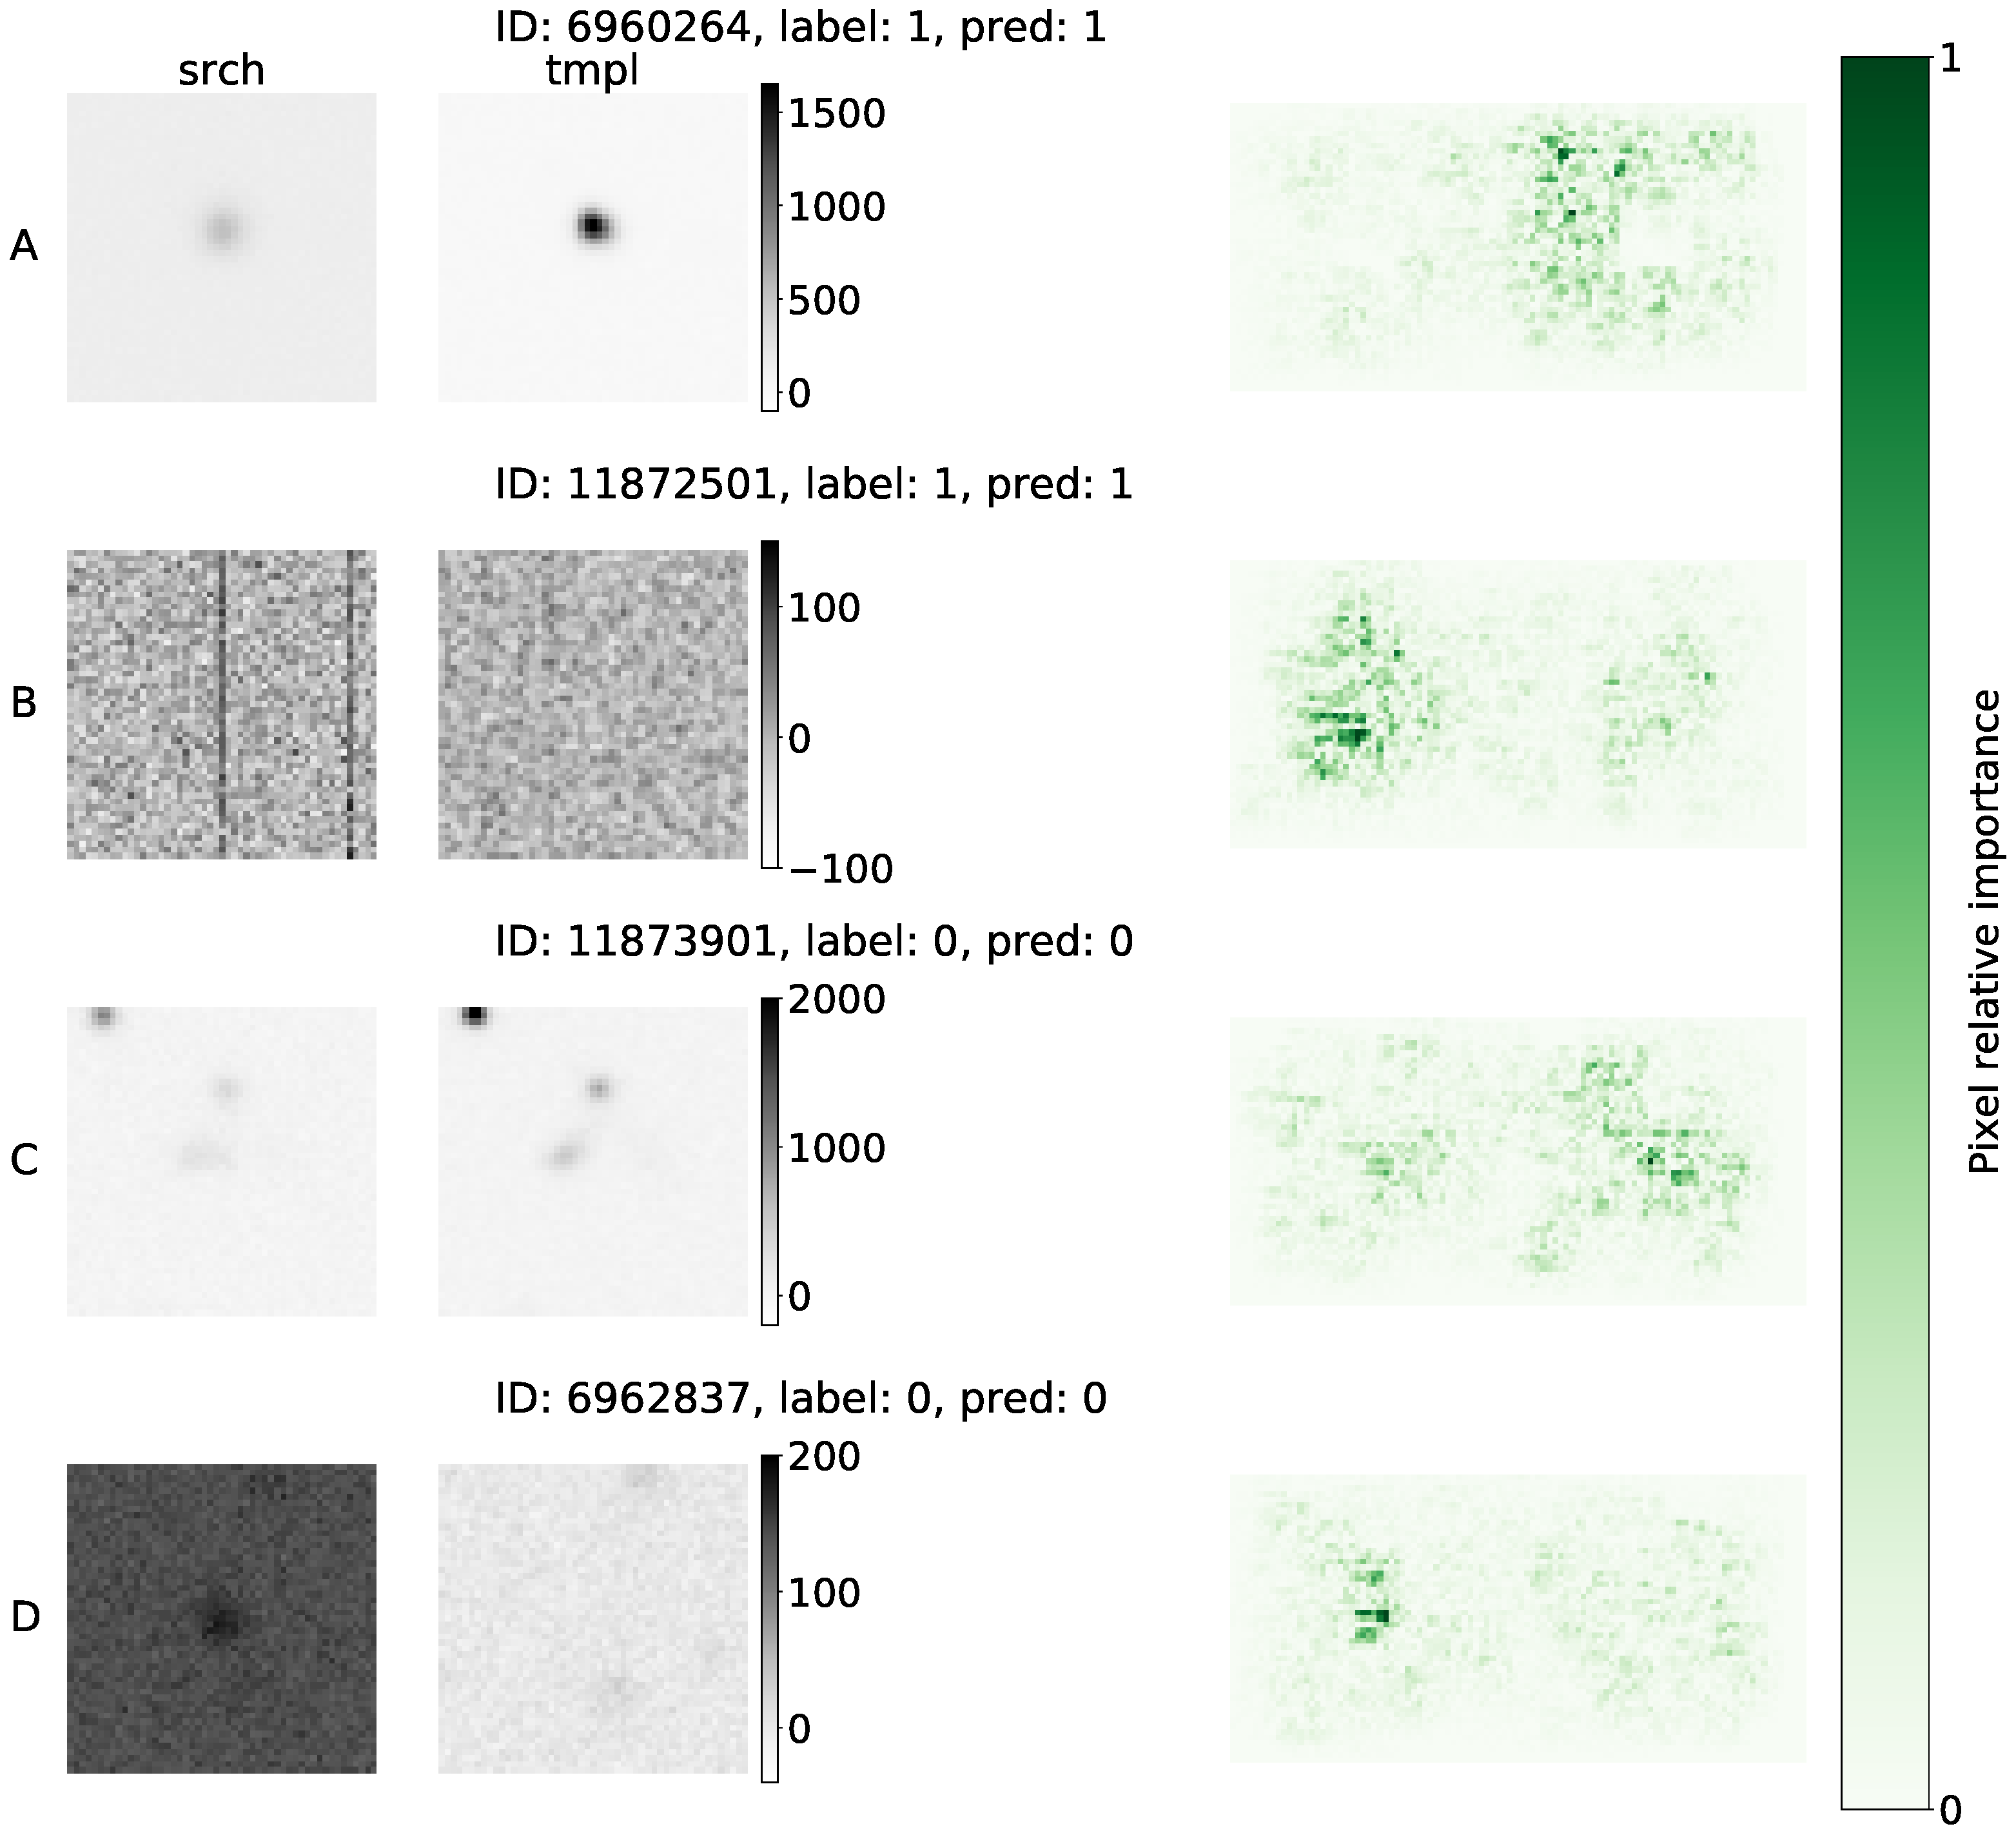
\includegraphics[width=0.84\linewidth]{
    figures/saliency_plot_noDIA.pdf}
    \caption{As \autoref{fig:saliency_4id} but for the \nodia\ model: saliency map for the four transients in \autoref{fig:examples_no_normalization}. This figure is discussed in more detail in \autoref{subsec: saliency}.}. 
    \label{fig:saliency_4id_noDIA}
\end{figure*}


% \begin{figure*}
% \begin{minipage}[b]{0.45\linewidth}
%     \centering
%     \includegraphics[width=1\linewidth]{
%     figures/ROC3D.pdf}
%     \caption{ROC curve for the $20,000$ images used for testing the \textbf{\diabased\ }model. The area under the curve was $0.992$.}
%     \label{fig:roc_modelAAA}
% % \end{figure}
% \end{minipage}
% \begin{minipage}[b]{0.45\linewidth}
% % \begin{figure}[H]
%     \centering
%     \includegraphics[width=1\linewidth]{
%     figures/ROC.pdf}
%     \caption{ROC curve for the $20,000$ images used for testing the \textbf{\nodia\ }model. The area under the curve was $0.973$.}
%     \label{fig:roc_modelCCC}
%     \end{minipage}
% \end{figure*}
\subsection{A peek into the model decisions through saliency maps}\label{subsec:results_seliancy}


% \masao{This is a very interesting section!  For readers like me who don't know much about how saliency maps are produced, can you write a couple of sentences about how they are made?  I think you said something about removing each pixel and looking at how much the predictions change.  A short description is helpful for the uneducated reader like me.}



\begin{figure*}
        \centering
    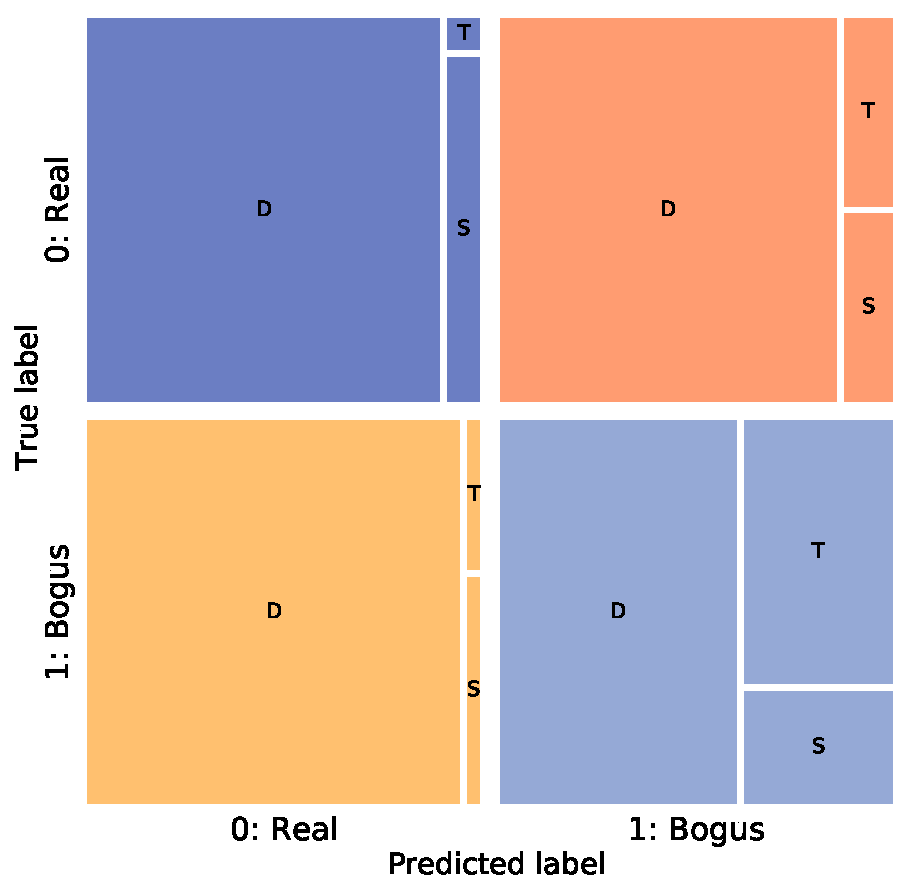
\includegraphics[width=0.45\linewidth]{
    figures/confusionmatrix_saliencyDIA_new.pdf}
     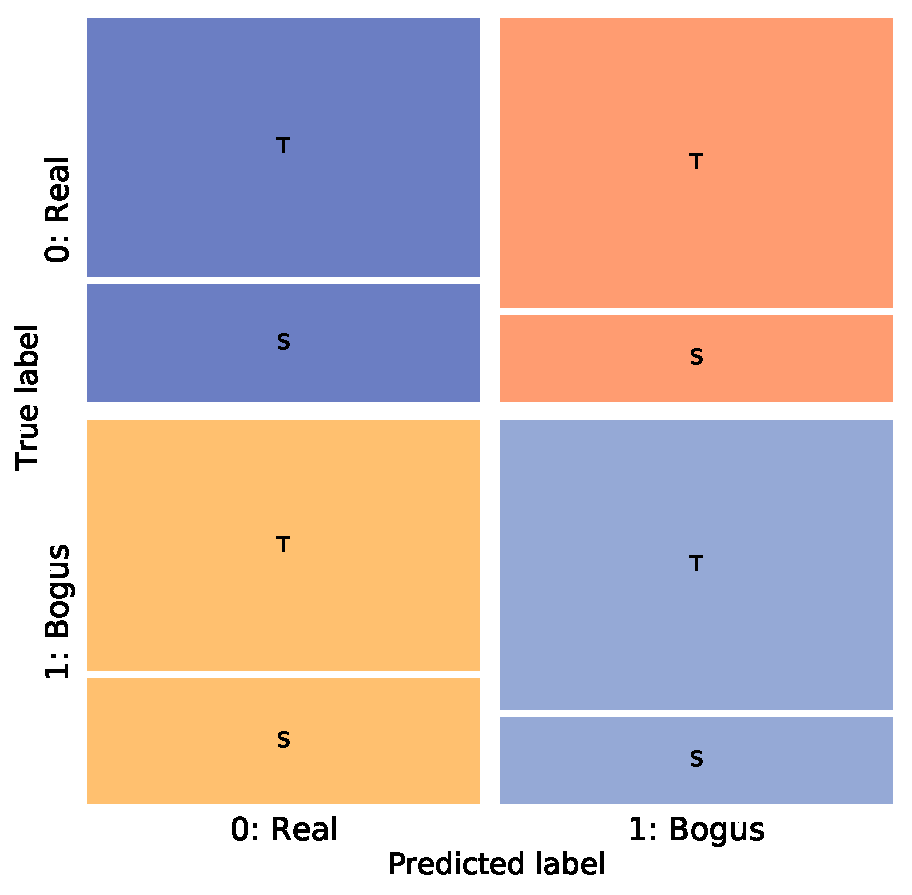
\includegraphics[width=0.45\linewidth]{
    figures/confusionmatrix_saliencynoDIA_new.pdf}
    \caption{Confusion matrix reporting the proportion of transients for which the highest concentration of important pixels is found in the \diff, \search, or \temp\ portion of the input image for the \diabased\ model results (left) and \nodia\ model (right), {\it Left}: \diabased. For 90\% ($8630$) of the $9564$ transients classified correctly as ``real'', the classification principally relied on the the \diff\ image ($I_\diff > 1/3$); for 9\% ($847$) on the the \search ;  and for 1\% ($87$) on the the \temp . For incorrect ``real'' classifications 86\% of the images relied principally on \diff\, 7\% on \search, and 7\% on \temp. For incorrect ``bogus'' classifications 95\% of the images relied principally on \diff\, 3\% on \search, and 2\% on \temp. For correct ``bogus'' classifications 61\% of the images relied principally on \diff\, 12\% on \search, and 27\% on \temp. {\it Right}: \nodia. Of the $9163$ transients classified correctly as ``real'', for 68\% of them, the classification relied principally on the \temp\ image. For the incorrect ``real'' and correct ``bogus'' classifications 76\% of the cases were principally based on the \temp. For the incorrect ``bogus'' classifications 66\% of the cases were principally based on the \temp. }
    \label{fig:saliency_confusions}
\end{figure*}

%A gradient of the final output with respect to the input data is the operation used to calculate the score. 
%A saliency map provides a score to each one of the pixels that form the image used for training the CNN base on how important is that pixel to the final classification of the CNNs. A gradient of the final output with respect to the input data is the operation used to calculate the score. 
%For the purpose of this work the score range is not relevant, we focus only on the value given by the code and that a higher value implies a more relevant pixel for the classification. A higher score of a pixel would indicated that a small change in that flux value would affect the final output, and consequently the final classification decision. 
%Our expectation is that pixels scored highly are located in the object that we want to classify. 

\begin{figure*}
    \centering
    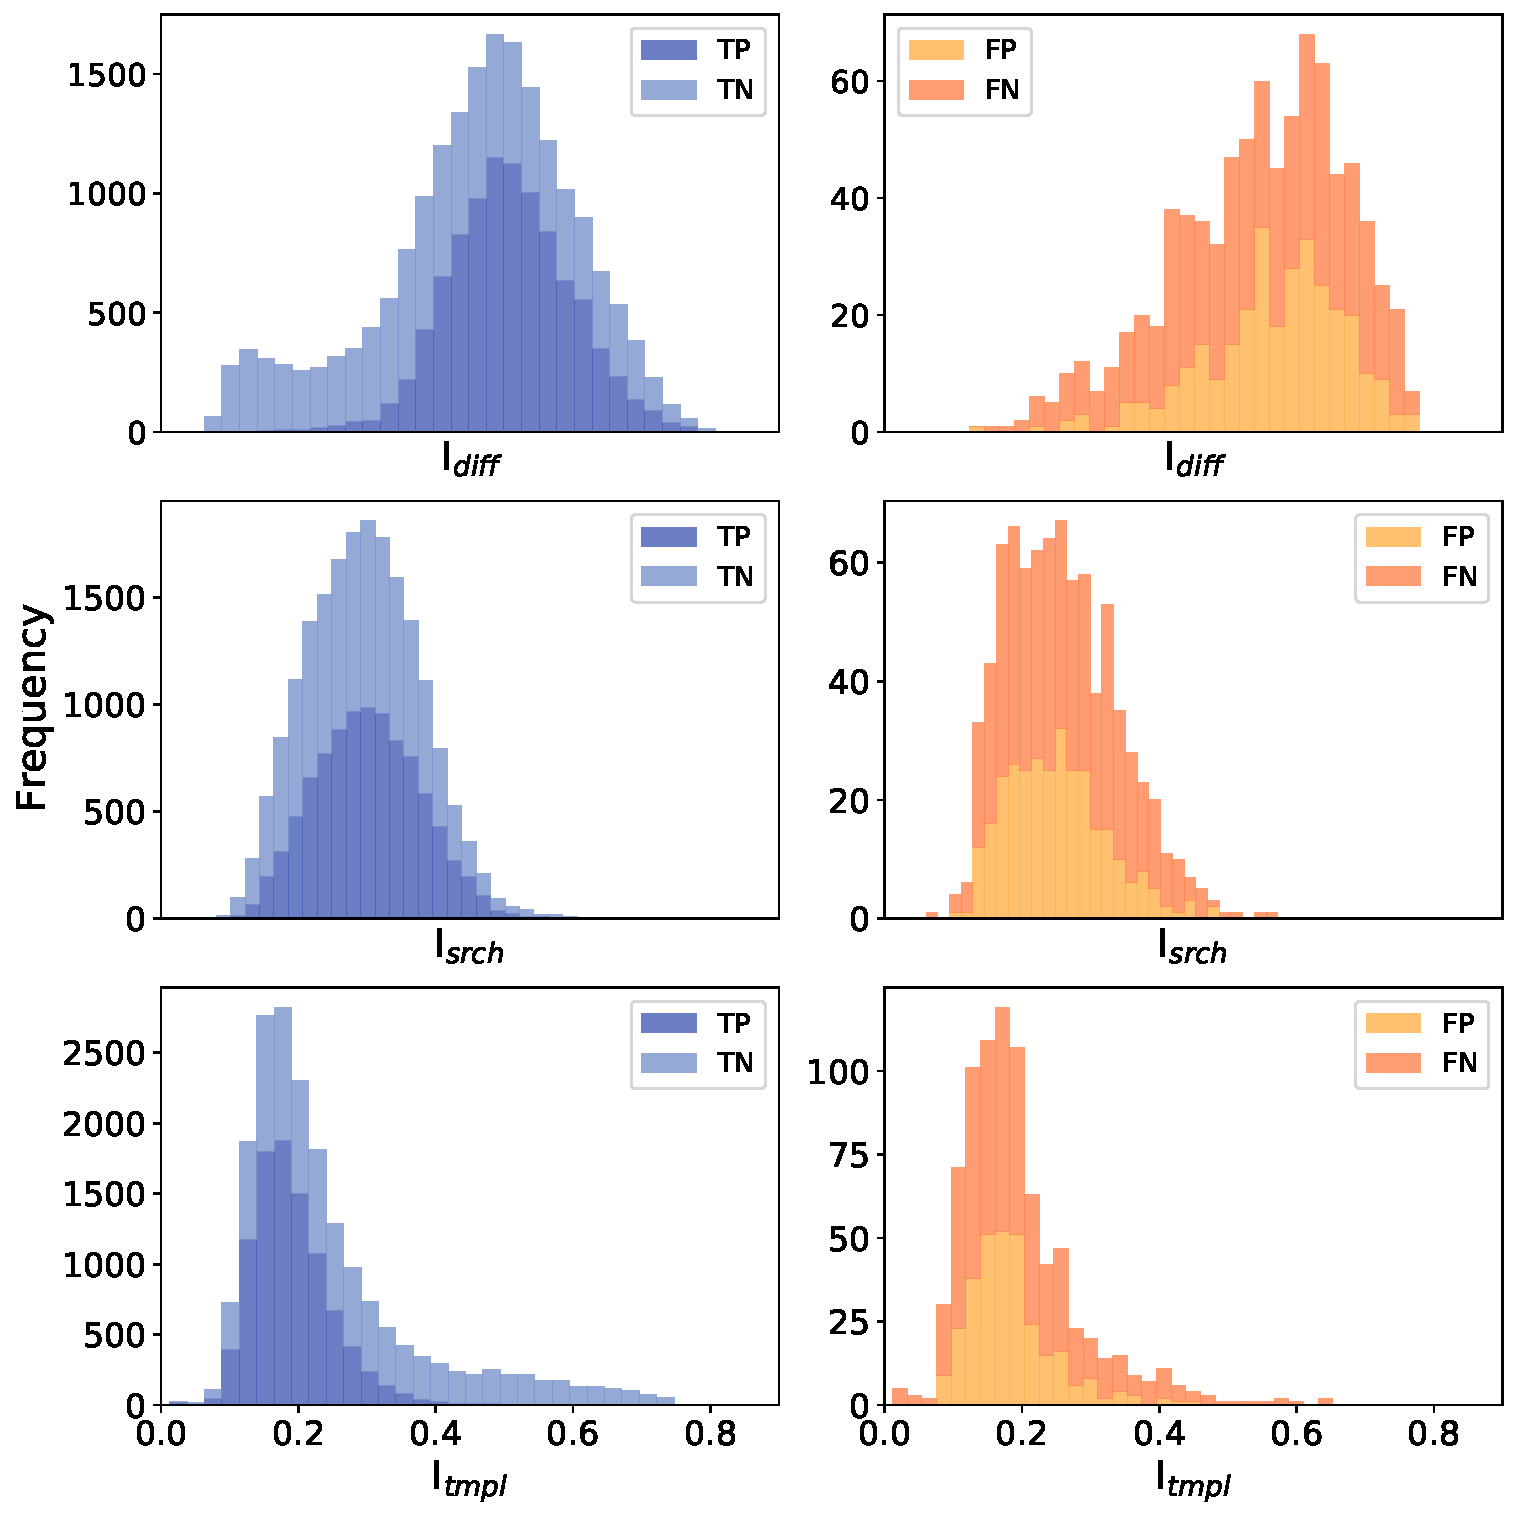
\includegraphics[width=0.45\linewidth]{
    figures/histogram_sm_important_pixels_fed_shared.pdf}
    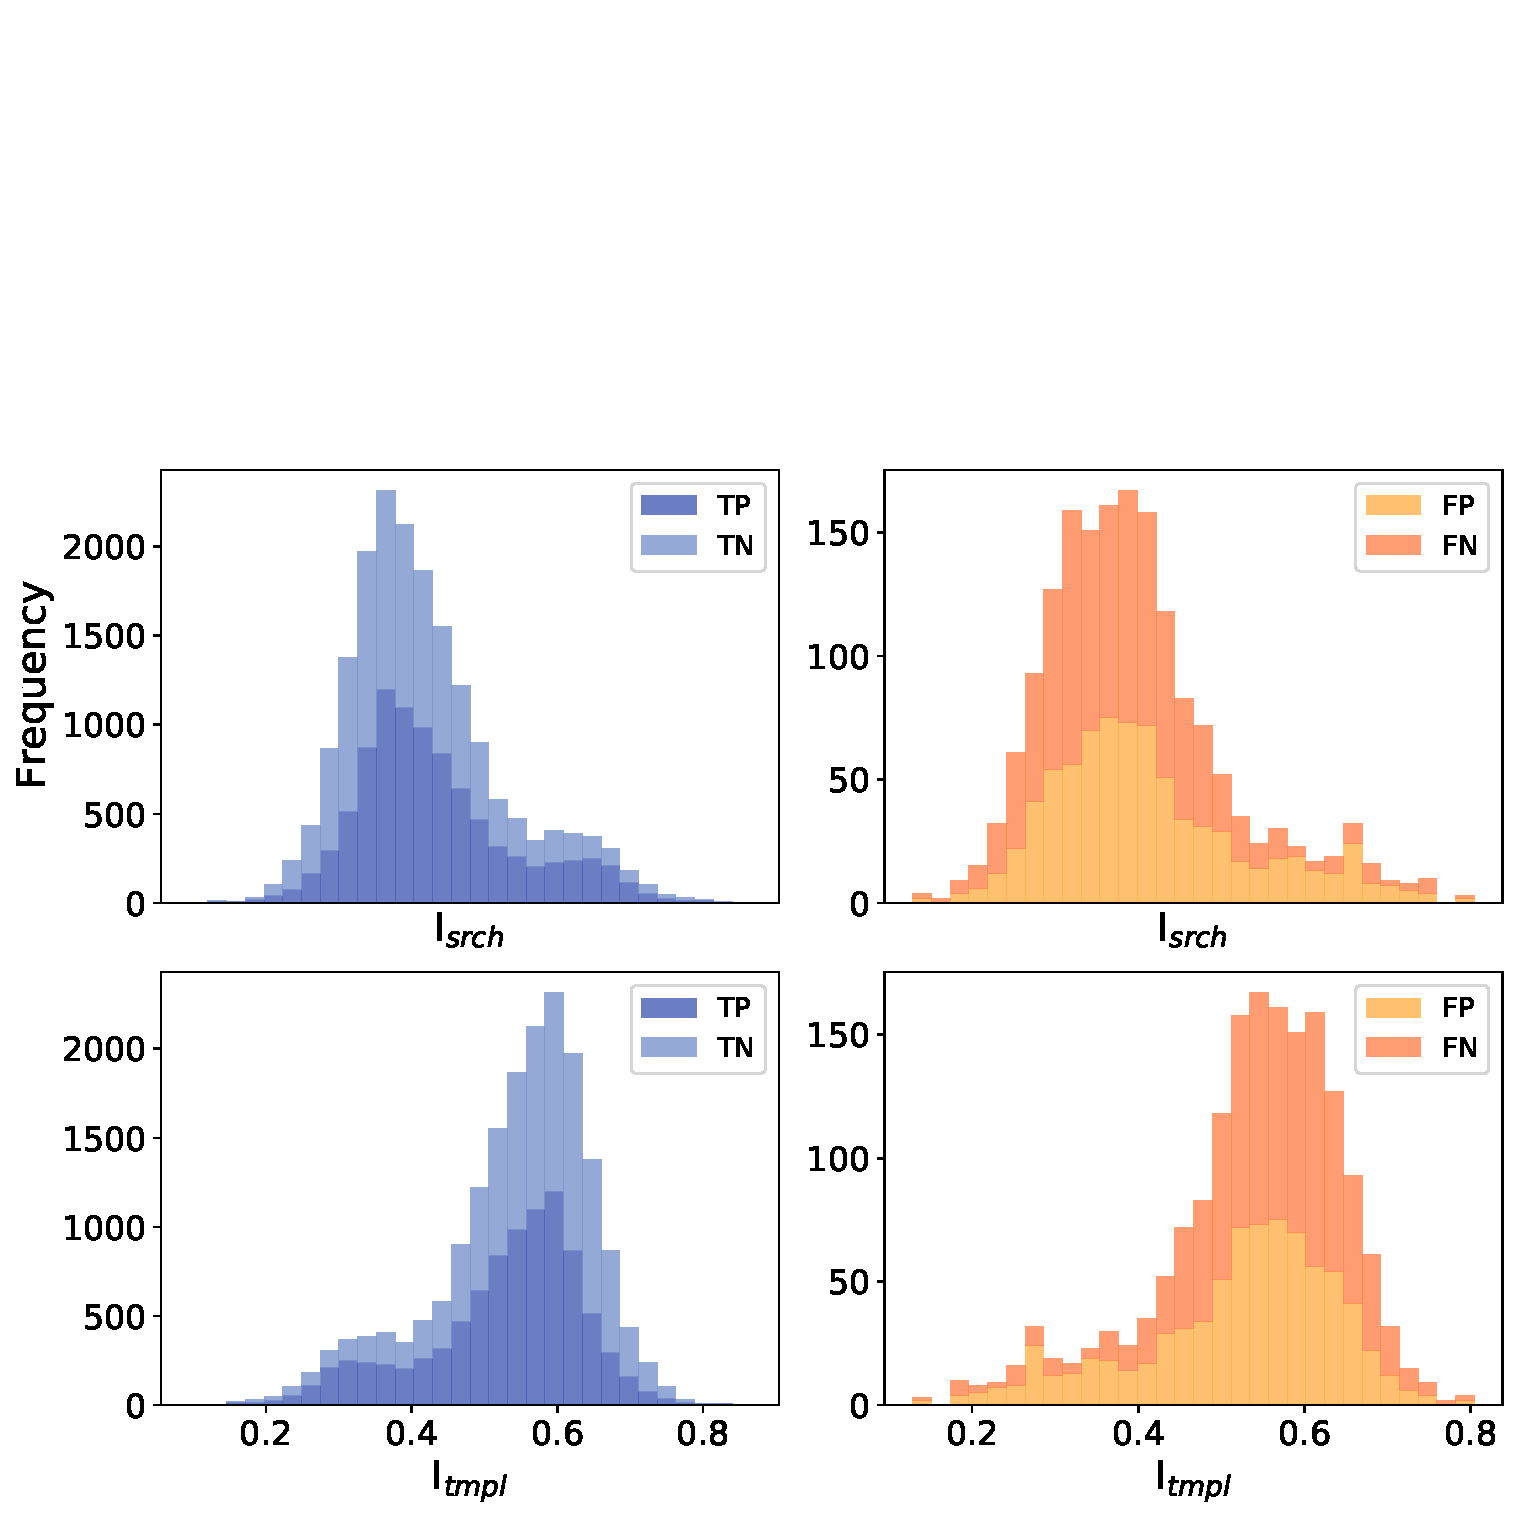
\includegraphics[width=0.45\linewidth]{
    figures/histogram_sm_important_pixels_2d_fed_shared.pdf}
    \caption{The distribution of  $\idiff$ (top), \isearch\ (middle), and \itempl\ (bottom) value for the 20,000 transients in the test data (see \autoref{eq: saliencymetric}). The colors corresponds to the quadrants of the confusion matrix to which the transient belong according to the model prediction, \diabased\ predictions in the first and second column from the left to the right and \nodia\ in the third and fourth. Blue shades correspond to correct predictions (TP and TN) and orange to FP and FN. Note that the $y$ axis values are different in each plot and the that FP and FN histograms contain far fewer observations. On the {\itempl Left}, for the \diabased\ model, the TP classification shows a preference for the \diff\ images and the distribution peaks at $\idiff \sim 0.5$. For TN, however, small $\idiff$ values are more common, with an significant fraction of observations in the $0<$\idiff$<0.33$ region. This behaviour is complemented by a long \itempl tail in the TN distribution ($0.4<\itempl<0.8$). The FP and FN distributions are qualatively similar to the TP and TN, but noisier, as they contain fewer than 10\% of the objects. {\it Right}: \nodia\ model. All four classes have qualitative similar distributions in \itempl and \isearch. Classifications rely mostly on the \temp\ in all cases ($\itempl > 0.5$)}
    \label{fig:histo_saliency}
\end{figure*}


In \autoref{subsec:scaling}, we described how the importance of individual image pixels in the RB prediction performed by our models can be measured, and the design of a saliency-based metric to assess which component of the image is most important to perform the RB classification. Here we inspect the saliency maps, both visually and quantitatively through the measured values of \idiff, \isearch, and \itempl. 


In \autoref{fig:saliency_4id} and \autoref{fig:saliency_4id_noDIA} we show the four transients we considered as examples throughout this work, the same images used in \autoref{fig:examples_no_normalization} and \autoref{fig:examples_hstack_normalization}, and the corresponding saliency maps for the \diabased\ model and \nodia\ model respectively. \autoref{fig:saliency_confusions} and \autoref{fig:histo_saliency} report the results of \autoref{eq: saliencymetric} for the objects in our training set.

Lets start with some considerations about the saliency maps for the four image examples for the \diabased\ model (\autoref{fig:saliency_4id}), and specifically from  panels C and D were the transients were correctly predicted as ``real''. We observe that the greatest concentration of important pixels for both these images is found in the left-most third of the image: %the \diff\ section, \question{approx the 50\% of all the pixels that form the triple in the saliency map}, meaning that
$\idiff \sim 0.5 $ for both. 
%, according to the definition in \autoref{eq: saliencymetric}.
We speculate, from our experience in labeling real/bogus by visual inspection and consulting with some of the human scanners that labeled the original \texttt{autoscan} images, that this behaviour is similar to what a human scanner would do: if in the \diff\ image there is a clearly real transient, the scanner would not need to study in detail the \search\ and \temp\ images. 

\autoref{fig:saliency_4id}A and B show correctly classified ``bogus'' transients. In \autoref{fig:saliency_4id}A, a ``bogus'' produced likely by a moving object displaying a classical dipole, the majority of the important pixels are located in the \temp\ ($\itempl \sim 0.54 $), concentrated around the location of the central source and the location  where its ``ghost'' image is (the coordinates corresponding to the location the bright patch of pixels in the \diff, but in the \temp\ portion of the composite image).
In \autoref{fig:saliency_4id}B, there is no central source and the detection is triggered by an image artifact. The important pixels are found in all three image segments and are spread around a large area of each image: the model has inspected the image in its entirety to decide the classification. 
Following our consideration about the similarity between the CNN and human decision process, we speculate that here too the CNN  mimics closely what a human scanner would do: because there is not a clear central source (a ``real'' object) in the \diff, the scanner would analyze the \search\ and \temp\ images to extract more information from the context to enable a classification. However, it should be noted that no quantitative studies of the features the human scanners use to classify transients has been done, thus this remains simply an intriguing suggestion.



For the case of the \nodia\ model, the expectation was less clear: both the \search\ and the \temp\ images are necessary to ``reconstruct'' the information contained in the \diff, and while the pixels overlapping with the central transient are obviously expected to be important, the pixels that surround it are necessary to essentially reproduce the scaling and PSF-matching operations between \temp\ and \search\ that the DIA performs. 
Accordingly, the saliency maps presented in \autoref{fig:saliency_4id_noDIA} are more difficult to interpret: in all four cases, important pixels are found all over the composite images.
%the results, that are presented graphically in right \autoref{fig:histo_saliency} and right \autoref{fig:saliency_confusions}, are more difficult to interpret.

To explore how the choice of important pixels may depend on the image label and on the correct classification we report  the fraction of images for which the \diff\ (\search, \temp) is the dominant source of important pixels {\it within} the confusion matrix in \autoref{fig:saliency_confusions}. To do this, we use a rough but intuitive cutoff: if the normalized sum of the saliency pixels in a third of the image is larger than $\frac{1}{3}$, then we deduce that the model principally used that component for its decision. For example, where $\idiff > 0.33$, we conclude that the model principally relied on \diff\ to make the RB classification. With this cut-off we can assess if there are differences in the model behavior when classifying objects as a function of their labels or their classification.
In all four cases (all combinations of ``real'' and ``bogus'' label and prediction) the concentration of important pixels is largest in the portion of the image corresponding to the \diff\  in the \diabased\ model. It is however interesting to note that, in order to correctly classify the ``bogus'', the \diabased\ model uses the template and search image more heavily than in all other cases (\diff, \search, \temp,  = 61\%, 12\%, 27\% for TN, while $I_\diff>85\%$ for TP, FP, and FN). 

The cut-off method described above does not allow us to distinguish between cases where multiple sections of the images were used jointly, perhaps with similar importance, from cases where the model truly only relied on one section of the image. For that, we take a closer look at the distribution of saliency values. 
In \autoref{fig:histo_saliency} we show the distribution of values of the three metrics defined in \autoref{eq: saliencymetric} for each of the four cases: TP and TN, in shades of blue, FP and FN, in shades of orange, following the color-scheme adopted in \autoref{fig:confusiomatrix_models} and \autoref{fig:saliency_confusions}. For the \diabased\ model (the two left-most columns), for the majority of the 20,000 images in the training set $\idiff > 0.33$, but there is a secondary pick in the $\idiff$ distribution near $\idiff \sim0.1$ populated entirely by TN cases, complementary to a long right tail in the \itempl distribution ($\itempl > 0.4$). This confirms that the correct classification in the presence of real transients relies on \diff, but \temp\ and \search\ become important to correctly classify bogus transients, just like we had seen in the exemplary cases in \autoref{fig:saliency_4id}. We note also that the general shape of each distribution (\idiff, \isearch, \itempl) is similar for the TP and TN case (blue) and for the FP and FN cases (orange). 
 
For the \nodia\ model the important pixels are concentrated in the \temp\  for most images ($\itempl > 0.5$) for both correct and incorrect classifications.
This is somewhat counter-intuitive since the \temp\ {\it does not} contain the transient itself! However, one may speculate that this is because the \temp, a higer quality image, contains more accurate information about the context in which the transient arises: \eg, if it is located near a galaxy or not. This information is important to the classification. It is also interesting to note that for the transients predicted as ``real'' in both TP and FP, the fraction of images that leveraged primarily the \temp\ is approximately $2/3$, and for images predicted as ``bogus'', in both TN and FN, it is approximately $3/4$.

To help guide the interpretation of the saliency maps, a few more maps are plotted in \hyperref[sec:appendixc]{Appendix C}. Where we provide 6 examples per each class of the confusion matrix, for both the \diabased\ and the \nodia\ models. 

\subsection{Computational cost of our models}\label{sec:computationcost}
The computational cost of our models, reported in CPU Node hours in \autoref{tab:acc results}, confirms that while training a CNN model for RB can be computationally expensive, and significantly more so if the \diff\ is not used in input (\nodia), the model prediction is instantaneous. Using a NN-based platform, the computational costs are front-loaded. In transient detection this could mean that the observation-to-transient discovery process is instantaneous, while computation time can be spent during off-sky hours (principally to build templates). Furthermore, while the training time is longer for the \nodia\ model than for the model that uses the \diff\ in input (\diabased) the computational cost of the forward-pass (prediction) scales superlinearly with the size of the feature set (pixels), so that our \nodia\ model takes less than half the time than the \diabased\ one to perform the RB task. With a clock time of 0.3 ms per 51$\times$51 pixels postage stamp, predicting over the full DES focal plane would take $\sim 1$ minute. However, we note that at this stage of our work we still rely on the DIA in several ways: while the \temp\ and \search\ in input to \nodia\ are not PSF matched, this proof of concept is performed on transients that were detected in \diff\ images, and we leverage the alignment of \temp\ and \search\ and centering of the postage stamp that arose from the DIA (see \autoref{sec:futurework}). Conversely, predictions would only need to be done in correspondence of the sources detected in the \temp\ and \search\ images, and not for the entire CCD plane.




% \begin{figure*}
% \begin{minipage}[b]{0.45\linewidth}
%     \centering
%     \includegraphics[width=0.8\linewidth]{
%     figures/confusionmatrix_saliencyDIA(1).pdf}
%     \caption{Confusion matrix and the proportion of the most important pixels given by the saliency map of each of the images in the triple after the training using the \textbf{\diabased\ }model. i.e., from the $9564$ transients classified correctly as ``real'', 90\% ($8630$) of them, the classification was done based principally on the \diff\ image due to the fact that the sum of pixels in the \diff\ section in the saliency map was the greatest of the three. }
%     \label{fig:saliency_confusionDIA}
% \end{minipage}
% \begin{minipage}[b]{0.45\linewidth}
%     \centering
%     \includegraphics[width=0.8\linewidth]{
%     figures/confusionmatrix__saliencynoDIA.pdf}
%     \caption{Confusion matrix and the proportion of the most important pixels given by the saliency map of each of the images in the duplex after the training using the \textbf{\nodia\ }model. i.e., from the $9147$ transients classified correctly as ``bogus'', 24\% ($2197$) of them, the classification was done based principally on the \search\ image due to the fact that the sum of pixels in the \search\ section in the saliency map was the greatest of the two. }
%     \label{fig:saliency_confusionnoDIA}
%     \end{minipage}
% \end{figure*}




